\documentclass[11pt]{article}

% Core packages (order matters: hyperref should load near-last to avoid
% clobbering other packages' commands).
\usepackage[T1]{fontenc}
\usepackage[margin=1in]{geometry}
\usepackage{graphicx}
\usepackage{booktabs}
\usepackage{amsmath}
\usepackage{xcolor}
\usepackage{caption}
\usepackage{hyperref}

\hypersetup{
  colorlinks=true,
  linkcolor=blue,
  urlcolor=blue,
  citecolor=blue,
  pdftitle={WTI Volatility- and Inventory-Regime Trading Research},
}

\newcommand{\todo}[1]{\textcolor{red}{\textbf{[TODO: #1]}}}
\newcommand{\provisional}[1]{\textcolor{orange}{#1 \textit{(provisional)}}}

\title{WTI Volatility- and Inventory-Regime Trading Research \\ \large Working Report}
\author{}
\date{\today}

\begin{document}
\maketitle

\begin{abstract}
This report documents an ongoing research project to build a systematic WTI
crude oil trading strategy. The project began as an inventory-driven
calendar-spread (CL1--CL2) mean-reversion model, and has since expanded to
incorporate geopolitical risk (GRI) and implied-volatility (OVX) signals,
with the current direction being a forward-looking volatility-regime model
intended to time entries into long-volatility options exposure ahead of
geopolitical escalation. This is a living document, updated as the
methodology evolves; sections marked \emph{provisional} reflect
work-in-progress that has not yet been fully validated.
\end{abstract}

\tableofcontents

% =====================================================================
\section{Introduction}
% =====================================================================

\subsection{Objective}
The original goal was to determine whether Cushing, Oklahoma crude
inventory levels provide a stable enough fair-value anchor for the WTI
CL1--CL2 calendar spread to support a profitable systematic trading
strategy. That question has since broadened in two directions:

\begin{enumerate}
  \item Whether geopolitical risk (proxied by a GRI index) and implied
  volatility (OVX) improve the fair-value model and risk management of the
  spread strategy.
  \item Whether a distinct, forward-looking \emph{volatility-regime} model
  --- using GRI as a leading indicator for OVX regime transitions --- can
  support a long-volatility options strategy that enters ahead of, and
  exits ahead of the resolution of, geopolitical escalation episodes.
\end{enumerate}

\subsection{Data}
The underlying dataset (\texttt{Misc.xlsx}) contains four daily/weekly
series:

\begin{itemize}
  \item \textbf{CL1, CL2}: front two NYMEX WTI futures contract settlement
  prices, daily, 2007--present.
  \item \textbf{Cushing inventory}: EIA weekly crude stock level, thousand
  barrels.
  \item \textbf{OVX}: CBOE Crude Oil Volatility Index, daily, available
  from 2007-05-10.
  \item \textbf{GRI}: a geopolitical risk index, daily (including
  non-trading days), 2007--present.
\end{itemize}

\paragraph{Data quality note.} During ingestion we identified that the most
recent $\sim$1{,}100 rows of the GRI date column (covering 2023-07 through
the present --- precisely the period containing the most significant
episode in the dataset) were stored as raw Excel serial numbers rather than
formatted dates. Naive parsing silently misread these as
1970-01-01-plus-nanoseconds, which would have caused those dates to sort to
the start of the series and the true recent GRI values to be lost from the
no-lookahead join (backward-filled with a stale mid-2023 value instead).
This is corrected in \texttt{load\_data.py} by detecting bare numeric date
values and converting them via the Excel epoch (1899-12-30) rather than
relying on pandas' default parser.

% =====================================================================
\section{Part I: Calendar-Spread Fair-Value Model}
% =====================================================================

\subsection{Baseline: inventory-squeeze hyperbolic model}
The original model regressed the CL1--CL2 spread on Cushing storage
utilization $u = \text{inventory} / \text{capacity}$:
\[
\text{spread} = \beta_0 + \frac{\beta_1}{u} + \frac{\beta_2}{1-u} + \varepsilon
\]
fit by OLS on data through the training cutoff (2025-01-13), with the
period after held out as an out-of-sample backtest.

\textbf{Problem identified:} the out-of-sample utilization range (24--40\%)
sat almost entirely in the bottom 5\% tail of the training distribution
(train 5th percentile: 29\%). A hyperbolic term is least constrained by
data and steepest exactly where it is being extrapolated, causing the fair
value to diverge sharply from the actual spread out of sample.

\subsection{Rejected fix: detrended/standardized utilization}
An initial hypothesis was that a fixed storage-capacity denominator, held
constant across a decade of actual capacity changes, was biasing the
utilization measure. We tested replacing raw utilization with a causal,
trailing-window detrended/standardized version
($\text{inv\_zdev} = (\text{inventory} - \text{trailing mean}) /
\text{trailing std}$).

\textbf{Result: this made out-of-sample fit worse}, not better (test RMSE
2.27 vs.\ 1.83 for the plain-utilization baseline; bias $+1.09$ vs.\
$+0.06$). The mechanism: detrending relative to a chasing trailing baseline
caused a \emph{sustained} multi-month low-inventory regime to be
re-classified as ``the new normal'' rather than a genuine squeeze, and the
model missed the largest backwardation spike in the sample entirely
(predicting a slightly negative/contango fair value while the actual spread
hit \$9.20). This held across trailing-window lengths from 6 months to 4
years --- i.e.\ this was not a tuning problem but a structural one:
detrending discards exactly the information that matters during a
sustained squeeze.

\textbf{Conclusion:} plain utilization was retained as the working feature.

\subsection{Functional form: spline vs. hyperbolic}
Separately, we tested replacing the hyperbolic terms with a natural cubic
spline in utilization (same feature, different functional form). This made
negligible difference to in-sample or out-of-sample accuracy on the
realized data, but is retained because it cannot diverge unboundedly on
future extrapolation the way $1/u$ can.

\subsection{Adding macro features: OVX and GRI}
With OVX and GRI added to the workbook, we tested augmenting the
spline-on-utilization model with each variable.

\begin{center}
\begin{tabular}{lrrrr}
\toprule
Model & Test RMSE & Test bias & Spike-window RMSE & Spike mean fair value \\
\midrule
Storage only & 2.185 & +0.369 & 4.05 & 0.57 \\
Storage + GRI only & \textbf{2.089} & \textbf{+0.262} & \textbf{3.85} & \textbf{0.80} \\
Storage + OVX only & 2.400 & +0.587 & 4.47 & 0.01 \\
Storage + both & 2.289 & +0.477 & 4.25 & 0.25 \\
\bottomrule
\end{tabular}
\captionof{table}{Actual spike-window mean spread was 2.94 (max 13.94).}
\end{center}

\textbf{GRI helps on every metric; OVX hurts.} OVX's historical relationship
to the spread is dominated by demand-collapse volatility episodes (2014--16,
2020) where volatility spiked \emph{alongside a contango blowout}, not a
backwardation squeeze --- a single linear coefficient cannot distinguish
``fear of too little oil'' from ``fear of too much oil,'' and the fitted
sign ends up wrong for a supply-shock scenario. GRI does not have this
problem since it targets geopolitical/conflict risk specifically.

We further tested nonlinear (spline) and threshold specifications for the
GRI term; both plateaued at a modest improvement over the linear version
(test RMSE $\approx$2.02, spike-window mean fair value $\approx$0.97),
still far short of the actual spike magnitude. \textbf{Conclusion:} this is
close to the ceiling of what a smooth function of a global news-count index
can explain for what is essentially a single extreme tail event in the
sample; further chasing this gap risks overfitting to one episode.

\textbf{Working fair-value model:}
\[
\text{spread} \sim \text{spline}(u,\ df=4) + \text{spline}(\log(\text{GRI}),\ df=4)
\]

\begin{figure}[h]
  \centering
  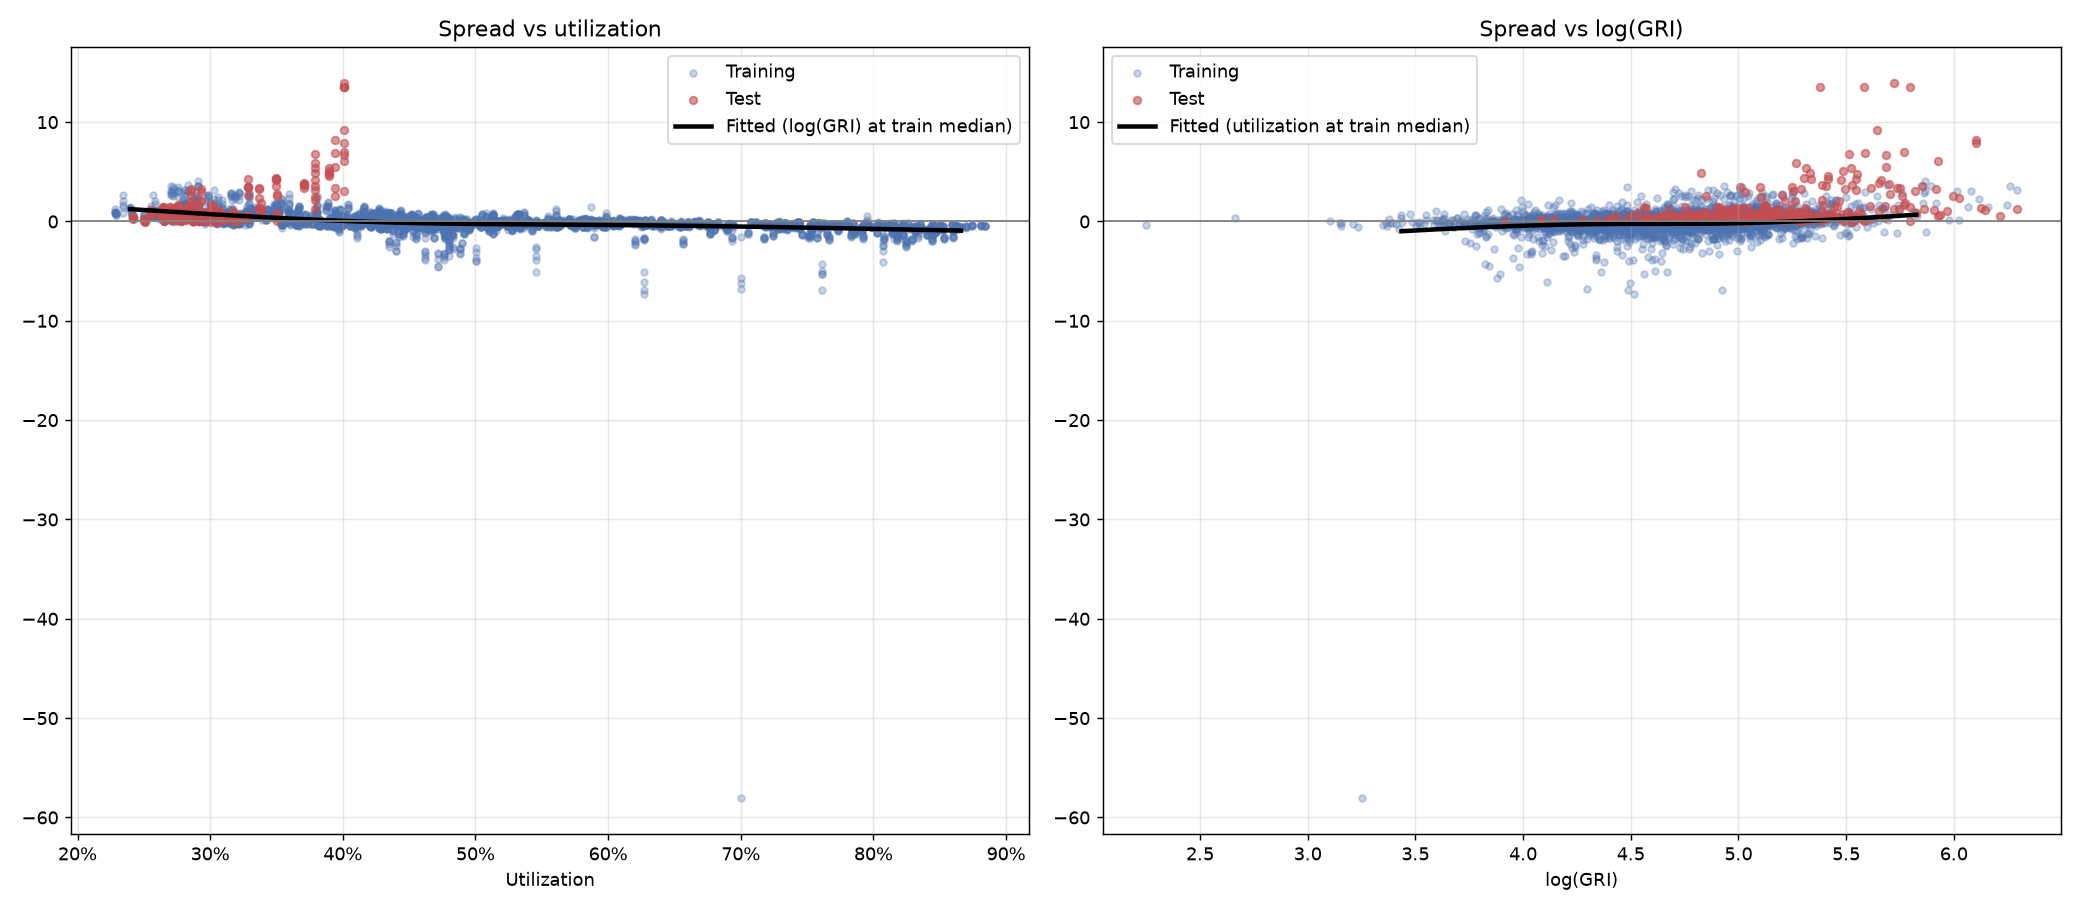
\includegraphics[width=0.95\textwidth]{../charts/01_fair_value_curve.png}
  \caption{Fitted fair-value curve vs.\ each input, training and test
  observations shown separately.}
\end{figure}

\begin{figure}[h]
  \centering
  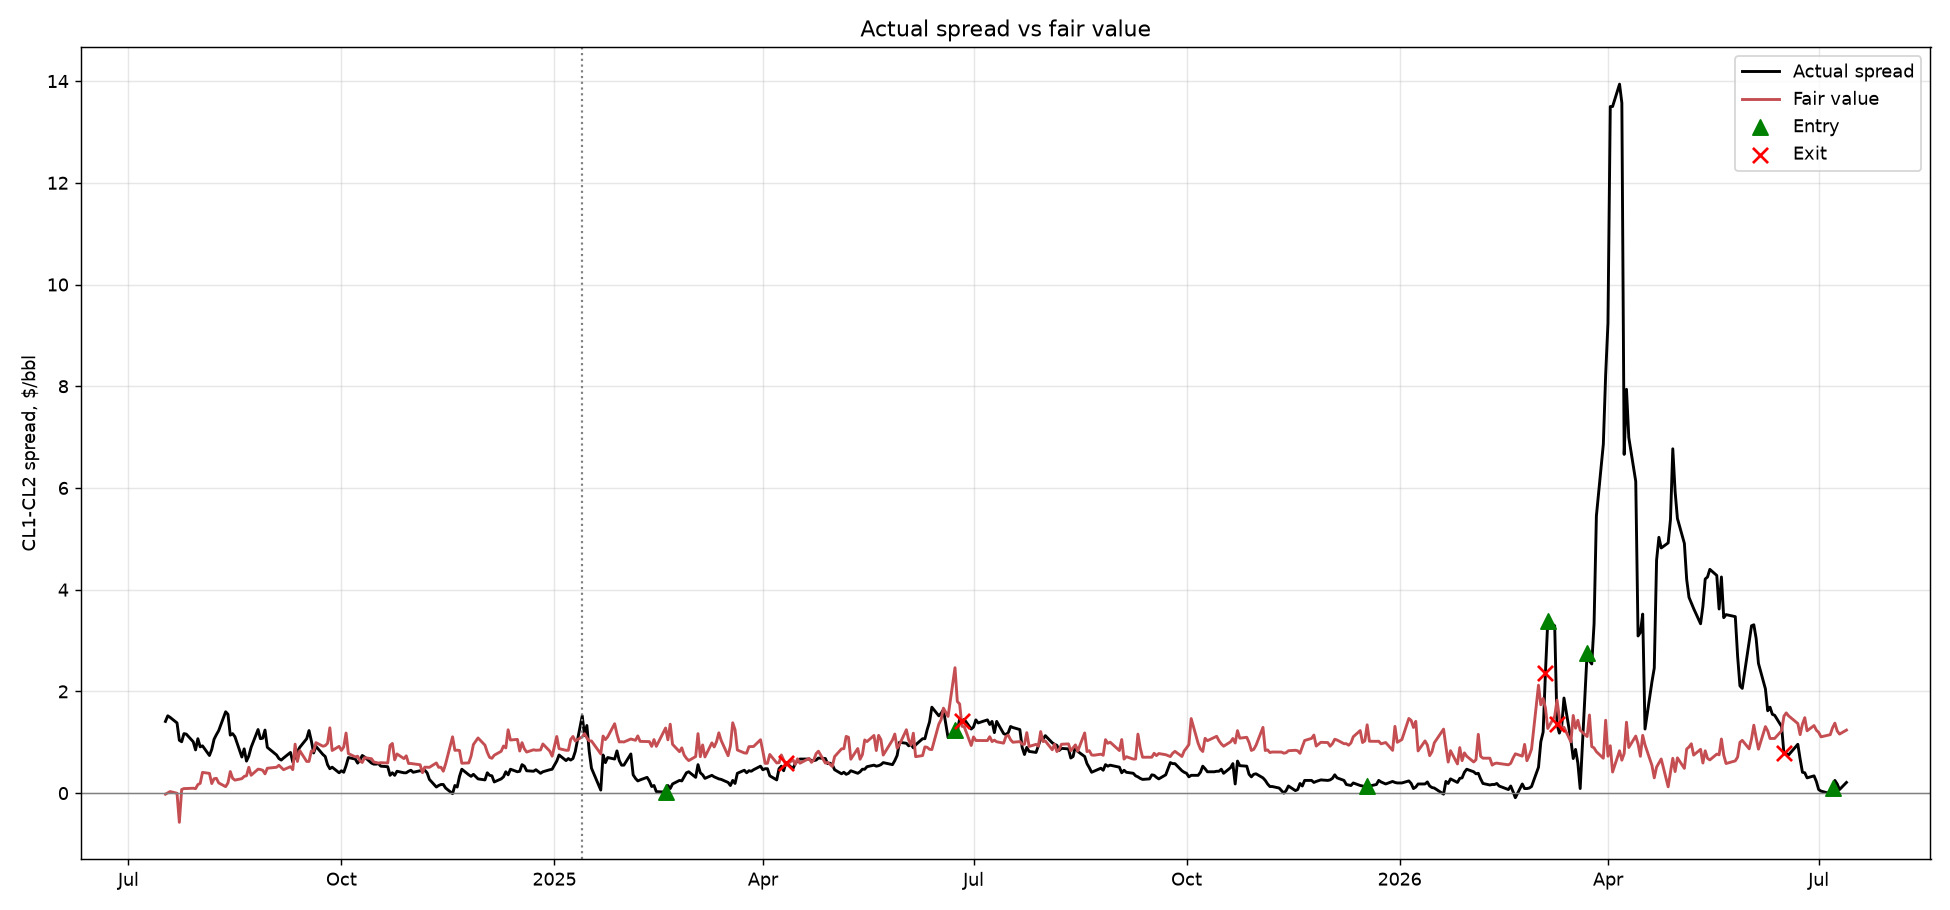
\includegraphics[width=0.95\textwidth]{../charts/02_actual_vs_fair_value.png}
  \caption{Actual spread vs.\ fair value over time, with strategy
  entries/exits marked.}
\end{figure}

% =====================================================================
\section{Part II: Regime Modeling}
% =====================================================================

\subsection{GRI-only regime classifier (Markov-switching, fixed transition matrix)}
A first regime model fit a Markov-switching model directly on
$\log(\text{GRI})$ to classify calm vs.\ crisis states, intended to gate new
spread-strategy entries during elevated-risk periods.

\textbf{Finding:} a 2-state fit classified \textbf{93.6\% of the entire
2025--2026 out-of-sample window} as ``crisis.'' This was not a modeling
artifact --- GRI has been structurally elevated across nearly the whole
window relative to the 2010--2025 training average, not just during the
acute March--June 2026 episode. A 3-state fit did not materially change
this (top-state mean essentially unchanged). A hard entry block based on
this classification was therefore judged too blunt (it would suppress
trading almost entirely), motivating continuous position-size scaling
instead of a binary gate for the spread strategy (Part III).

\subsection{\provisional{Forward-looking vol-regime model (TVTP)}}
The current direction reframes the problem: rather than classifying
\emph{today's} state from GRI, fit a Markov-switching model on
$\log(\text{OVX})$ --- the volatility series we actually want to trade ---
where the \textbf{transition probabilities are themselves a function of
GRI} (time-varying transition probabilities, TVTP). When GRI rises, the
model's own probability of transitioning into the high-volatility state
rises too, in principle \emph{before} OVX has necessarily moved, which is
what allows a genuine multi-day-ahead forecast rather than a same-day
classification.

\paragraph{Mechanism.} Given the filtered state distribution at time $t$ and
the GRI-conditioned transition matrix $T_t$, the $h$-day-ahead state
forecast is $T_t^h \cdot p_t$ (Chapman--Kolmogorov), under the simplifying
assumption that today's GRI level persists over the forecast window (we
cannot know future GRI). Forecast horizons of 3, 5, 10, and 15 trading days
are computed.

\paragraph{State-count experiments.}
\begin{center}
\begin{tabular}{lll}
\toprule
States & Converged? & Notes \\
\midrule
4 & No & Well-separated means (20.6/31.3/44.5/81.8); good qualitative behavior but unreliable given non-convergence. \\
3 & No & Over-triggered: crisis probability reached 99.5\% by 2026-02-19 (OVX only 56.7), far too early. \\
2 & \textbf{Yes} & Means 29.2/48.7. Passes sanity checks: correctly low ($<$1\%) in genuinely calm historical windows (mid-2017, early 2024); intermediate ($\sim$54\%) during mid-2019, which coincides with real Gulf-of-Oman tanker-attack tensions that year. \\
\bottomrule
\end{tabular}
\end{center}

Convergence was achieved by standardizing (not just centering) the GRI
regressor in the TVTP specification and adding a BFGS polish step after the
initial EM/search-based fit.

\paragraph{Preliminary single-episode read.} Examining daily resolution
around the 2026-03-02 GRI spike (to 500.8) in isolation initially suggested
the forecast only reacts same-day with GRI, offering lead time only over
OVX completing its own move. The full validation below (across all
historical episodes, not just this one) shows a more favorable picture.

\subsection{Validation across all historical high-volatility episodes}
Every OVX$>$60 episode since 2007 (25 in total, identified by grouping
consecutive high-OVX days) was used as a validation set. For each episode,
we compare the $h$-day-ahead \emph{forecast} ($\text{crisis\_prob\_fwd}h$)
computed exactly $h$ trading days \emph{before} the episode's onset ---
i.e.\ the forecast a trader would actually have had in hand in advance,
using only information available at that earlier date --- against a
calm-period baseline (mean forecast during OVX$<$35 days).

\textbf{Methodological caveat:} 19 of the 25 episodes occurred before
\texttt{TRAIN\_END} (2025-01-13) and were therefore part of the training
data; strong performance there is chiefly an in-sample fit-quality check.
Only the 6 post-cutoff episodes (2025-06-17 and all four 2026 episodes) are
a genuine out-of-sample test, and are reported separately.

\begin{center}
\begin{tabular}{lrr}
\toprule
Horizon $h$ (trading days) & OOS episode mean forecast & Calm-day baseline \\
\midrule
3  & 0.961 & 0.032 \\
5  & 0.864 & 0.045 \\
10 & 0.902 & 0.074 \\
15 & 0.867 & 0.100 \\
\bottomrule
\end{tabular}
\end{center}

\textbf{Result: a real, substantial lead-time signal.} Even 15 trading days
(three calendar weeks) before an actual OVX$>$60 spike, the out-of-sample
forecast averaged $\approx$87\% crisis probability, against a $\approx$10\%
baseline. All 25 episodes were eventually detected (peak
$\text{crisis\_prob\_now}$ $\approx$100\% during the episode itself), and
the false-positive rate is low: during genuinely calm days (OVX$<$35),
only 0.99\% show $\text{crisis\_prob\_now} > 0.5$ (mean 1.24\%).

\paragraph{Honest limitation: genuine surprises are not forecastable.} Two
episodes --- \textbf{2011-08-09} (the sudden US credit-rating downgrade)
and \textbf{2021-11-26} (the Omicron variant announcement) --- showed
essentially \emph{no} anticipatory lift at any horizon (all four forecasts
remained near the 3--10\% baseline). Both were single-day news shocks with
no gradual build-up in GRI beforehand. This is an expected and honest
limitation, not a modeling failure: a leading indicator that only moves
once news breaks cannot forecast that news in advance. The model detects
\emph{escalating} situations (gradual GRI build-up ahead of a vol regime
shift, which describes most geopolitical/supply episodes including 2026),
not single-day surprise shocks.

\paragraph{Status: validated, ready for the next stage.} Given this
result, the 2-state TVTP model is considered validated as a regime
simulator. Remaining open items (Part V) are to (a) revisit whether 3/4
states can be made to converge with the improved optimizer settings, since
more granularity could sharpen the calm/elevated/crisis distinction, and
(b) define and backtest the actual entry/exit trading rule on top of this
now-validated forecast.

% =====================================================================
\section{Part III: Strategy / Risk Management (calendar-spread leg)}
% =====================================================================

\subsection{Original strategy and its failure mode}
Entries at $|z\text{-score}| \geq 1.0$, exits only on exact zero-crossing of
the residual, fixed 1-contract size, no stop-loss, no time stop.

\textbf{Result:} across the out-of-sample window, total P\&L of
\$3{,}470--\$7{,}100 (depending on fair-value model version) against a
\textbf{maximum drawdown of \$11{,}400} --- more than 3$\times$ total
profit. Root cause: a March 2026 SHORT position was held through the entire
war-fear spike (spread moving from 2.76 to 14.0 against the position)
because the exit rule only triggers on full mean-reversion, with no
mechanism to cut losses during an extended adverse move.

\subsection{Risk-management additions}
Four mechanisms were layered onto the base signal:
\begin{itemize}
  \item \textbf{Partial-convergence exit} ($|z|\leq 0.3$) rather than an
  exact zero-crossing, shortening average holding period.
  \item \textbf{Hard stop-loss} at $|z| \geq 3.0$, capping the ``ride an
  unbounded move'' failure mode directly.
  \item \textbf{Time stop} at 40 trading days, calibrated at roughly
  2$\times$ the weekly-resampled residual half-life ($\approx$20 trading
  days) --- the daily-resampled half-life ($<$1 day) reflects noise, not
  the structural convergence horizon.
  \item \textbf{Regime-based position sizing} (rather than a binary entry
  block, per the Part II finding above).
\end{itemize}

\paragraph{Iteration on the regime-sizing formula.} A naive linear size
$= 1 - \text{crisis\_prob}$ collapsed P\&L to near-zero (\$5), because
filtered regime probabilities from a persistent Markov model saturate near
0 or 1 almost everywhere rather than lingering at graded intermediate
values --- a linear scale crushes size almost all the time rather than
differentiating ``somewhat tense era'' from ``acute spike.''
\todo{A piecewise sizing curve (full size below a threshold, ramping to
zero only near the most extreme readings) was proposed but not yet
re-tested after the pivot to the forward-looking vol-regime model; revisit
once Part II is validated.}

\begin{figure}[h]
  \centering
  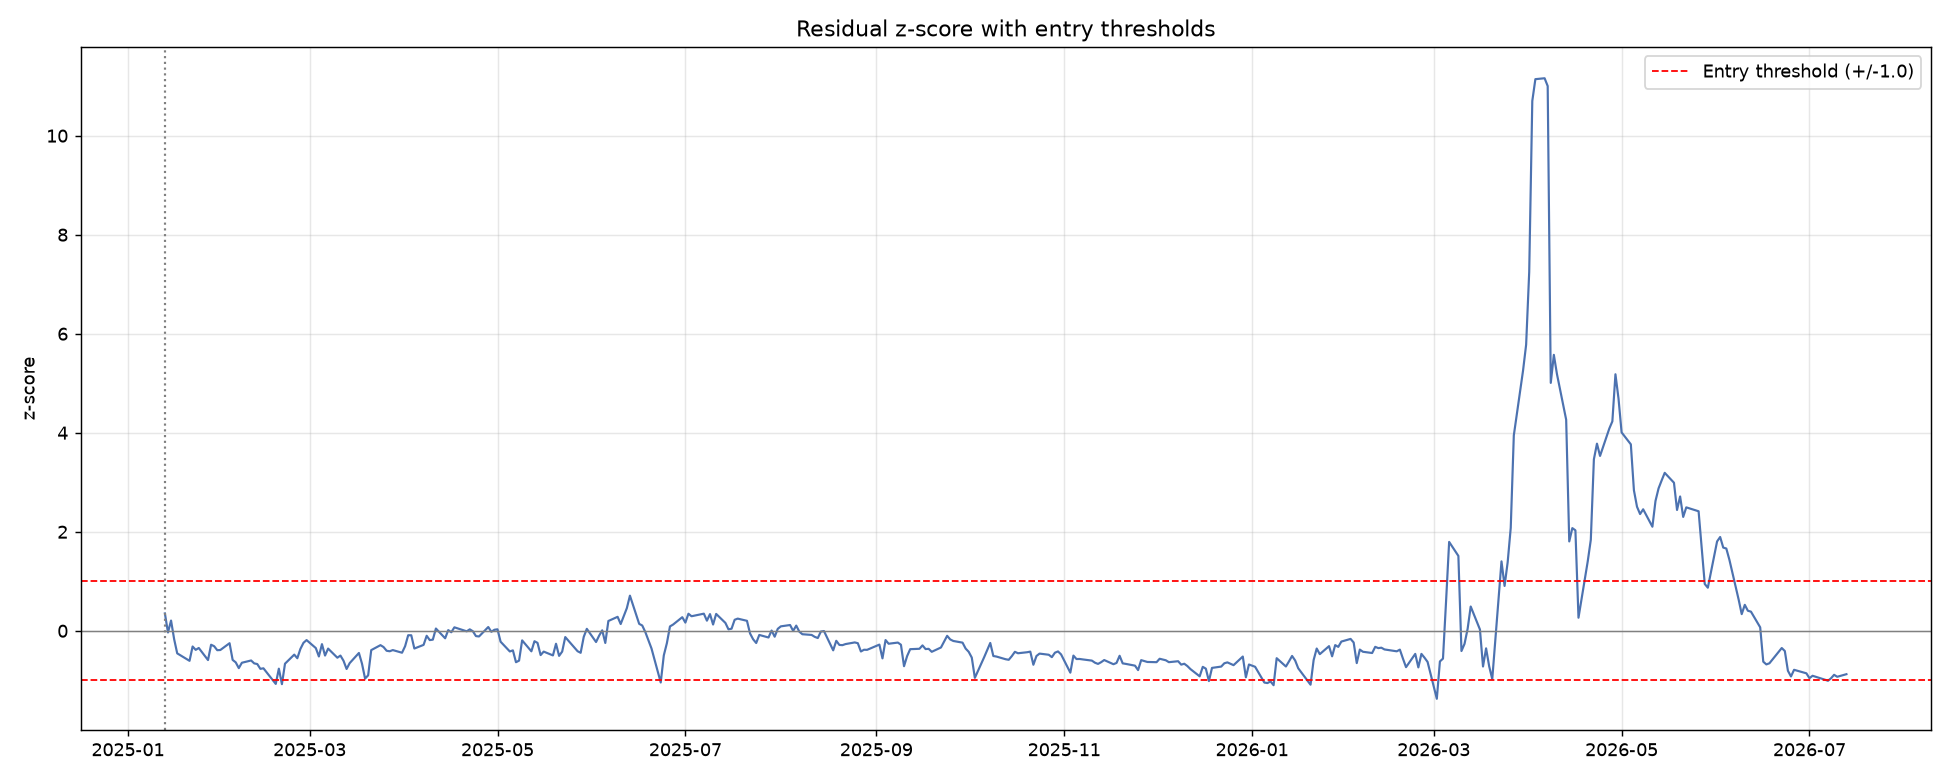
\includegraphics[width=0.95\textwidth]{../charts/03_zscore_bands.png}
  \caption{Residual z-score with entry thresholds.}
\end{figure}

\begin{figure}[h]
  \centering
  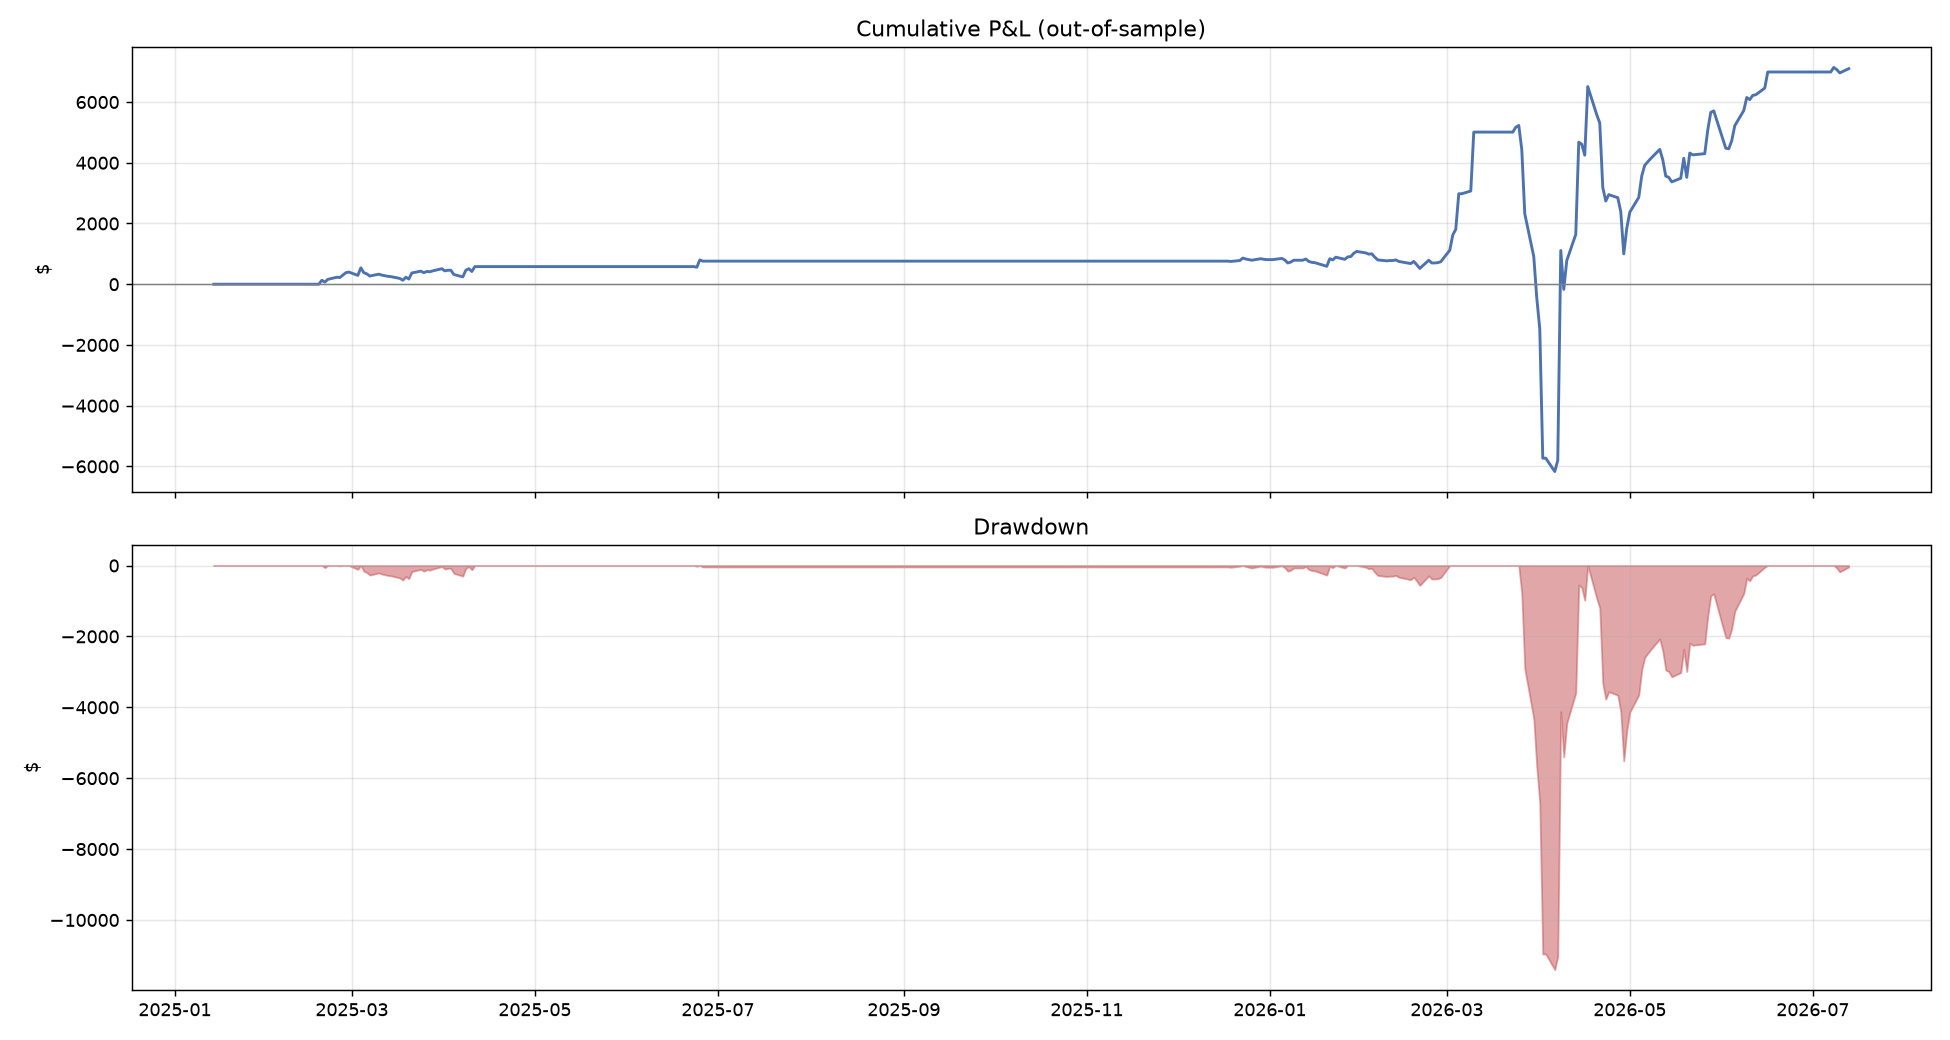
\includegraphics[width=0.95\textwidth]{../charts/04_pnl_drawdown.png}
  \caption{Cumulative P\&L and drawdown, out-of-sample.}
\end{figure}

% =====================================================================
\section{Part IV: \provisional{Volatility-Timing Options Strategy (new direction)}}
% =====================================================================

\subsection{Motivation}
Given that geopolitical escalation events (a) are poorly explained by the
inventory-squeeze spread model beyond a modest GRI adjustment, and (b) are
exactly the events that make the spread strategy's tail risk hardest to
manage, the current direction is a \emph{separate} strategy: use the
forward-looking vol-regime model (Part II) to time entries into
long-volatility options exposure (e.g.\ a straddle/strangle) ahead of a
regime transition into high volatility, and exit ahead of the transition
back to calm.

\subsection{Data constraint}
The dataset contains OVX (an aggregate implied-volatility index) but not an
actual option chain (strikes, expiries, per-strike IV, bid/ask). Two paths
were discussed for eventually backtesting P\&L:
\begin{enumerate}
  \item A variance-swap-style payoff proxy,
  $\text{P\&L} \propto \text{realized variance} - \text{OVX}^2$, requiring
  no strike/skew assumptions (the standard idealization of a delta-hedged
  straddle).
  \item A simplified Black-Scholes straddle using OVX as a flat implied-vol
  input.
\end{enumerate}
\textbf{Current status:} the regime simulator (Part II) is now validated
across all 25 historical episodes with a real, substantial out-of-sample
lead-time signal. Payoff modeling remains deferred; the entry/exit rule
(below) has now been defined and backtested on timing alone.

\subsection{Entry/exit rule (\texttt{vol\_strategy.py})}
A two-state (FLAT / LONG\_VOL) state machine, with no direction ambiguity
--- purely a decision of whether to hold vol exposure. \textbf{Design
revised 2026-07-16} after reviewing the first version's behavior (see
below); current design:

\begin{itemize}
  \item \textbf{Entry}: $\text{crisis\_prob\_fwd10} \geq 0.50$ (forecast-based,
  unchanged from the validated regime model in Part II -- enough lead time
  to execute an options trade before volatility re-prices).
  \item \textbf{Exit}: a level-based bracket on OVX itself, anchored to the
  OVX level \emph{at entry} (not a trailing peak): take profit if OVX rises
  25\% above entry, stop loss if OVX falls 25\% below entry. \textbf{No
  forecast dependency once in the trade.}
  \item Binary sizing (fixed size in/out) --- no continuous scaling yet,
  since no payoff model exists yet to calibrate a sizing dial against.
  \item Trading restricted to strictly after \texttt{TRAIN\_END}, consistent
  with the project's no-lookahead discipline.
\end{itemize}

\paragraph{Why the exit was redesigned.} The first version used a
forecast-based exit ($\text{crisis\_prob\_fwd5} \leq 0.20$), symmetric in
spirit to the entry. This waited for the model to confirm the crisis
regime was ending, which happens well after the actual peak: trade 1
entered at OVX$=$55.26, peaked at 71.56, but the forecast-based exit didn't
fire until OVX had round-tripped all the way down to 34.38 --- \emph{below
entry} --- giving back the entire gain. The level-based bracket fixes this
by locking in a defined outcome without depending on the forecast to decay
in time.

An intermediate design (flip directly from LONG\_VOL to SHORT\_VOL on the
same forecast-decay signal, harvesting the vol risk premium as things
calm down) was proposed and discussed but explicitly not implemented,
pending further design confirmation -- see \texttt{CLAUDE.md} for the
resulting standing rule to confirm major design changes before building
them.

\subsection{Timing backtest (no payoff attached yet)}
Since payoff modeling is deferred, the diagnostic here is whether the
\emph{timing} is directionally sound.

\paragraph{Methodological note (peak vs.\ average realized vol).} An
earlier version of the realized-vol diagnostic measured volatility as a
single average over the entire holding period, which produced a
misleading 0\% ``hit rate'' --- a long holding period dilutes a brief,
genuine vol spike into an unremarkable average (confirmed directly:
trade 1's average realized vol over its original 66-day hold was
$\approx$42.1, flat versus its entry level of 42.2, despite a real peak of
55.5 partway through). Replacing the average with the \emph{peak} trailing
realized volatility fixed this; the bracket-exit redesign below makes
holding periods much shorter regardless, so this matters less now.

\paragraph{Result: 14 trades, much faster turnover.} Because entry stays
armed as long as $\text{crisis\_prob\_fwd10} \geq 0.50$ (true for most of
an extended crisis window), the position re-enters immediately after each
bracket exit, producing a sequence of round-trips within a single
escalation episode rather than one long hold.

\begin{center}
\begin{tabular}{lr}
\toprule
Metric & Value \\
\midrule
Total / closed trades & 14 / 13 \\
Average holding days (median) & 13.8 (8) \\
Closed via take-profit & 53.8\% \\
Closed via stop-loss & 46.2\% \\
\bottomrule
\end{tabular}
\end{center}

A win rate above 50\% on a symmetric $\pm$25\% bracket is a promising
directional result, though not yet a P\&L figure (no payoff model
attached).

\paragraph{Known limitation of an entry-anchored (non-trailing) bracket.}
Trade 2026-03-09 to 2026-04-14 entered at OVX$=$100.53 and rose to a peak
of 120.91 during the hold (a large paper gain) but still closed as a
\textbf{stop-loss}, because OVX fell back to 75.35 -- more than 25\% below
the \emph{entry} level -- before the position was closed. An
entry-anchored bracket can convert a large intermediate gain into a
booked loss if price round-trips far enough; a trailing-stop-from-peak
variant would behave differently. Not changed for now since it wasn't
part of the confirmed design, but worth keeping in mind.

\todo{Sweep the take-profit/stop-loss percentages (currently 25\%/25\%,
untested against alternatives). Attach a payoff model (variance-swap proxy
or simplified Black-Scholes straddle) to convert this timing result into
an actual P\&L backtest. Consider whether a trailing-stop-from-peak
variant of the exit bracket is worth testing alongside the entry-anchored
version.}

\begin{figure}[h]
  \centering
  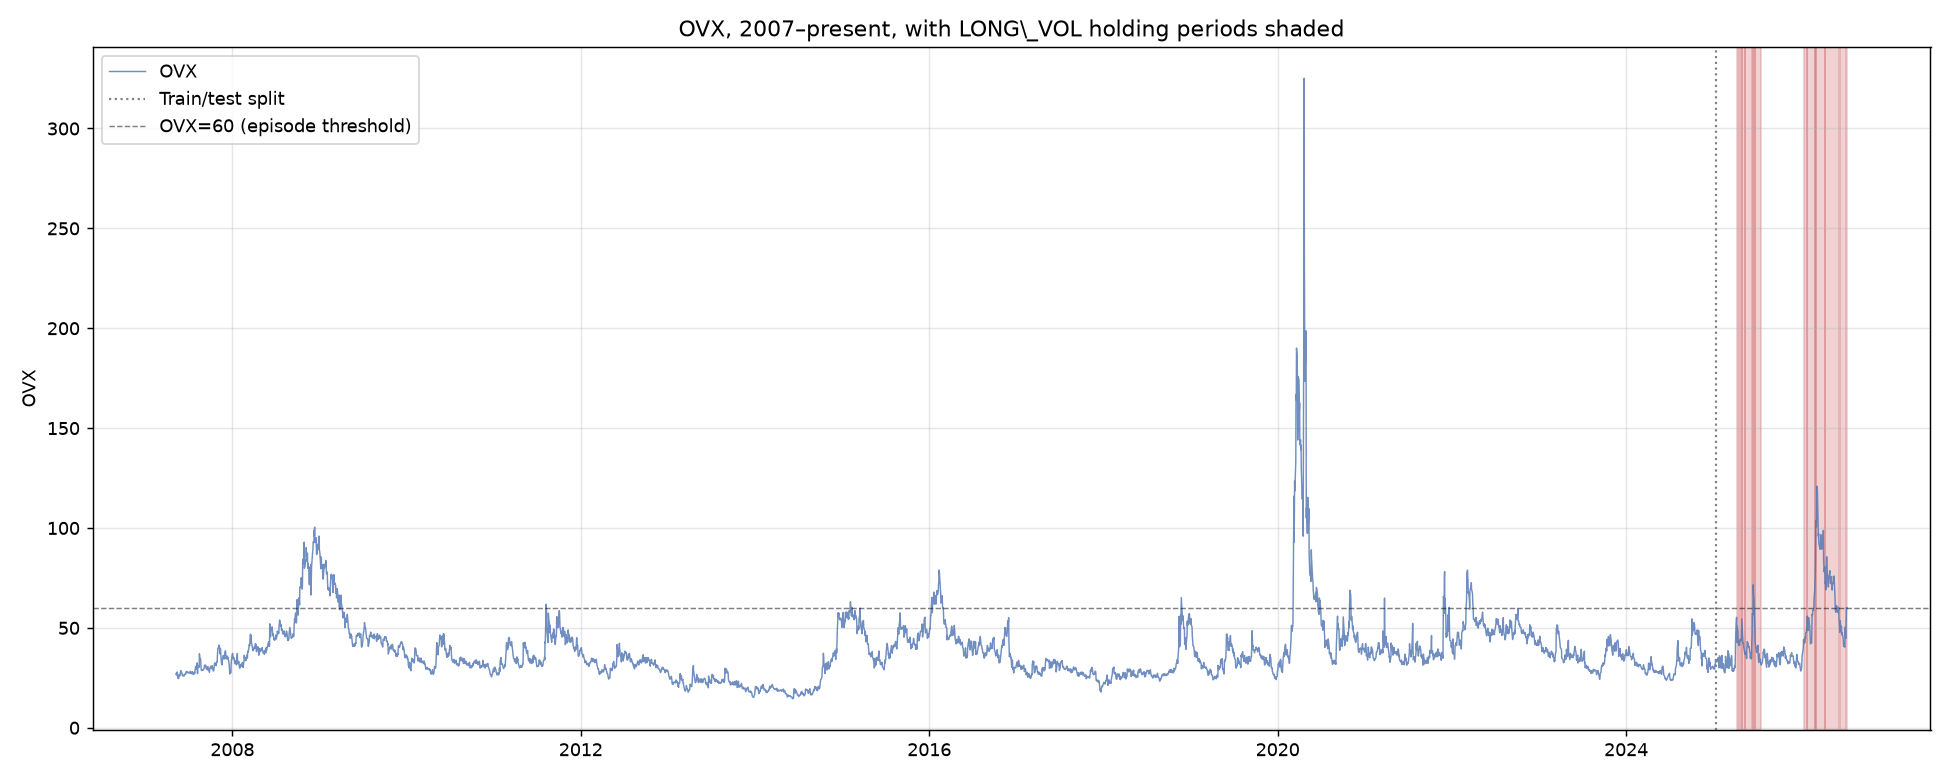
\includegraphics[width=0.95\textwidth]{../charts/05_vol_ovx_full_history.png}
  \caption{OVX, 2007--present, with LONG\_VOL holding periods shaded,
  shown against 19 years of history including 2008 and 2020.}
\end{figure}

\begin{figure}[h]
  \centering
  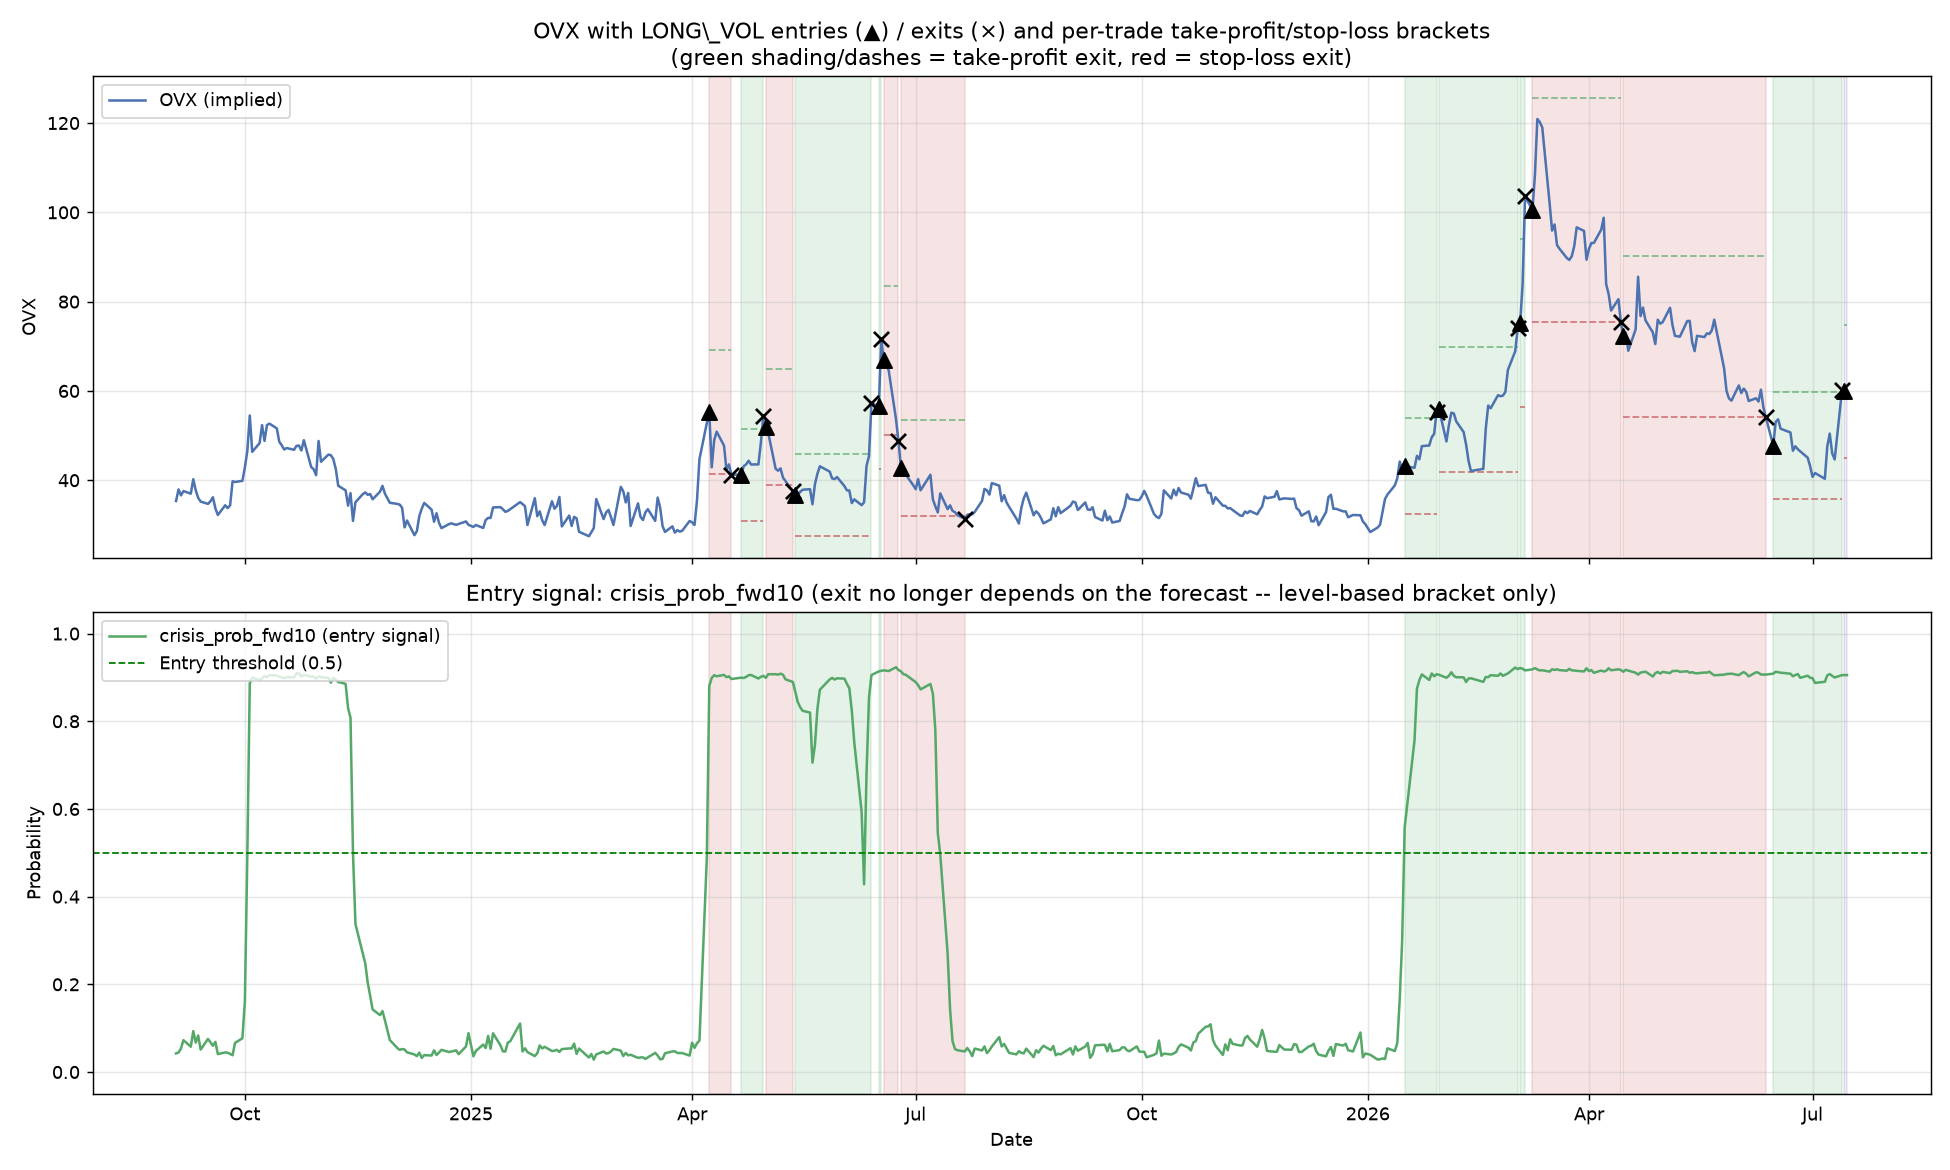
\includegraphics[width=0.95\textwidth]{../charts/06_vol_signal_detail.png}
  \caption{Top: OVX with entries (\(\triangle\)), exits (\(\times\)), and
  each trade's take-profit/stop-loss bracket levels (green/red dashed
  segments); shading indicates the realized outcome. Bottom: the entry
  forecast signal, which no longer drives exits.}
\end{figure}

% =====================================================================
\section{Summary of Open Items}
% =====================================================================
\begin{itemize}
  \item \textbf{[Done]} Validate the 2-state TVTP vol-regime model across
  all historical high-vol episodes: 87--96\% out-of-sample forecast
  probability at 3--15 day horizons vs.\ a 3--10\% calm baseline; genuine
  surprise shocks (2011 debt downgrade, 2021 Omicron) are, expectedly, not
  anticipated.
  \item \textbf{[Done, revised 2026-07-16]} Define and backtest the
  entry/exit rule for the volatility-timing strategy. First version
  (forecast-based exit) exited well after the peak, giving back entire
  gains; redesigned to a level-based $\pm$25\% OVX bracket anchored to
  entry. Result: 14 trades, 53.8\% take-profit / 46.2\% stop-loss, average
  8-14 day holding period. Payoff modeling still pending.
  \item \textbf{[Process change]} Added \texttt{CLAUDE.md} requiring
  explicit confirmation before major design changes to modeling/strategy
  logic, after an intermediate long/short-vol-flip design was proposed
  mid-task without being asked for.
  \item \todo{Attempt to recover a converged 3- or 4-state TVTP fit with the
  improved optimizer settings, for sharper calm/elevated/crisis granularity.}
  \item \todo{Sweep the take-profit/stop-loss bracket percentages, and
  attach a payoff model (variance-swap proxy or simplified Black-Scholes
  straddle) to convert the timing result into an actual P\&L backtest.}
  \item \todo{Consider a trailing-stop-from-peak variant of the exit
  bracket (vs.\ the current entry-anchored version) given the known case
  where a large intermediate gain round-tripped into a booked loss.}
  \item \todo{Revisit the discussed (not implemented) long/short-vol-flip
  idea as a distinct, explicitly-confirmed design if still wanted.}
  \item \todo{Re-derive a working regime-based position-sizing curve for
  the spread strategy using the now-validated vol-regime forecast (rather
  than the earlier, saturated GRI-only classifier).}
  \item \todo{Consider sourcing real historical WTI options chain data if
  the synthetic payoff proxy proves insufficiently realistic.}
\end{itemize}

\end{document}